%% ============================================================================
%%
%%  Speciale / Master's thesis
%%
%%  Author: FORNAVN EFTERNAVN
%%
%%  IMPORTANT: Compile with pdfLaTeX+biber !
%%
%%  Remarks:
%%  - Needs to be executed with '--shell-escape' if the minted-package is used!
%%
%%  Original template/preamble: Jakob Lysgaard Rørsted (Mosumgaard)
%% ============================================================================

% ~~~~~~~~~~~~~~~~~~~~~~~~~~~~~~~~~~~~~~~~~~~~~~~~~~~~~~~~~~~~~~~~~~~~~~~~~~~~~
% Preamble and input control
% ~~~~~~~~~~~~~~~~~~~~~~~~~~~~~~~~~~~~~~~~~~~~~~~~~~~~~~~~~~~~~~~~~~~~~~~~~~~~~

% Use memoir!!!
\documentclass[%
% final,           % Un-comment when finished (to e.g. remove watermark)
11pt,
openright,
twoside,
% danish,
british,
a4paper
]{memoir}

% Global definition: Name of the project (e.g. for the headers)
% NOTE: The text of the front page is defined manually!
\newcommand{\projecttitle}{Coffee Consumption by Students}
\newcommand{\projecttitledanish}{Studerendes Kaffeindtag}

% Read the actual preamble
%% ============================================================================
%%
%%  Master's thesis
%%
%%  Author: FORNAVN EFTERNAVN
%%
%%  Preamble
%%
%%  Original preamble: Jakob Lysgaard Rørsted (Mosumgaard)
%% ============================================================================

% ~~~~~~~~~~~~~~~~~~~~~~~~~~~~~~~~~~~~~~~~~~~~~~~~~~~~~~~~~~~~~~~~~~~~~~~~~~~~~
% Core
% ~~~~~~~~~~~~~~~~~~~~~~~~~~~~~~~~~~~~~~~~~~~~~~~~~~~~~~~~~~~~~~~~~~~~~~~~~~~~~
% Essentials
\usepackage[utf8]{inputenc}
\usepackage[T1]{fontenc}

% Microtype -- Subliminal refinements towards typographical perfection
\usepackage{microtype}
\microtypesetup{final}
% \microtypesetup{tracking = true}

% Various tools needed in the preamble and by some packages
\usepackage{etoolbox}

% Inclusion of code
% --> Needs to be loaded this early to avoid problems with some font packages
% NOTE: This packages requires the Python-module 'Pygments' to be installed
% NOTE: Fails unless this file is compiled with '--shell-escape' !
% \usepackage{minted}
% \usemintedstyle{friendly}

% Language (has to be loaded before the fonts..?)
% Load both languages to make two different abstracts
\usepackage[danish,english]{babel}
%\usepackage[danish,british]{babel}
\renewcommand\danishhyphenmins{22}
\selectlanguage{english}

% Fonts: Linux Libertine (http://www.tug.dk/FontCatalogue/linuxlibertine/)
\usepackage{libertine}            % Linux Libertine as text font
\usepackage{libertinust1math}     % Math support for Linux Libertine
\usepackage[scaled=.95]{newtxtt}  % Pretty teletype in correct size


% ~~~~~~~~~~~~~~~~~~~~~~~~~~~~~~~~~~~~~~~~~~~~~~~~~~~~~~~~~~~~~~~~~~~~~~~~~~~~~
% Page 'n' stuff
% ~~~~~~~~~~~~~~~~~~~~~~~~~~~~~~~~~~~~~~~~~~~~~~~~~~~~~~~~~~~~~~~~~~~~~~~~~~~~~
% Page set-up
\setlrmarginsandblock{3.2cm}{*}{1.5}
\setulmarginsandblock{*}{3.7cm}{1}

% Some memoir tricks
\setlength{\topskip}{1.6\topskip}
\checkandfixthelayout
\sloppybottom
\strictpagechecktrue

% To remove the blank page after the titlepage to save space
% --> Only for this progress report! Normally the blank page should be there!!
\usepackage{atbegshi}


% ~~~~~~~~~~~~~~~~~~~~~~~~~~~~~~~~~~~~~~~~~~~~~~~~~~~~~~~~~~~~~~~~~~~~~~~~~~~~~
% Page and chapter styles
% ~~~~~~~~~~~~~~~~~~~~~~~~~~~~~~~~~~~~~~~~~~~~~~~~~~~~~~~~~~~~~~~~~~~~~~~~~~~~~

% NOTE: Colors added everywhere, to make them easy to change!
\usepackage{xcolor}

% Fonts
\newcommand{\foliofont}{\color{black}\sffamily}
\newcommand{\headerfont}{\color{black}\sffamily}

% Make new pagestyle
\makepagestyle{jrmbsc}
\makeevenhead{jrmbsc}{\foliofont\thepage}    {} {\headerfont\leftmark}
\makeoddhead {jrmbsc}{\headerfont\projecttitle} {} {\foliofont\thepage}
\makeevenfoot{jrmbsc}{}{}{}
\makeoddfoot {jrmbsc}{}{}{}

% Black magic happens below! (define pagestyle)
\makeatletter
\makepsmarks {jrmbsc}{
  % Syntax: \createmark{<division type}{left|right|both marks}{shownumber|nonumber}{prefix}{postfix}
  \createmark{chapter}    {both}  {shownumber} {\@chapapp\ } {\ $\cdot$\ }
  \createmark{section}    {right} {shownumber} {}            { \ }
%  \createmark{subsection} {right} {nonumber}   {}            {}
  \createplainmark{toc}   {both}  {\contentsname}
  \createplainmark{lof}   {both}  {\listfigurename}
  \createplainmark{lot}   {both}  {\listtablename}
  \createplainmark{bib}   {both}  {\bibname}
  \createplainmark{index} {both}  {\indexname}
}
\makeatother
\nouppercaseheads

% Sections with sans-serif
\setsecheadstyle{\Large\bfseries\sffamily\raggedright}
\setsubsecheadstyle{\large\bfseries\sffamily\raggedright}

% Fix of the pagestyle of the chapter-pages
\copypagestyle{chapter}{empty}
\makeoddfoot{chapter}{}{\foliofont\thepage}{}
\makeevenfoot{chapter}{}{\foliofont\thepage}{}

% Chapterstyle (modified from Rasmus Villemoes thesis)
\usepackage{graphicx}
\makechapterstyle{jrmbsc}{% requires graphicx package
  \chapterstyle{default}
  \renewcommand*{\chapnamefont}{%
    \normalfont\LARGE\color{black}\scshape\raggedleft}
  \renewcommand*{\chaptitlefont}{%
    \normalfont\Huge\color{black}\sffamily\raggedleft}
  \renewcommand*{\chapternamenum}{}
  \renewcommand*{\printchapternum}{%
    \makebox[0pt][l]{\hspace{0.4em}
      \resizebox{!}{5ex}{%
        \normalfont\Large\color{black}\thechapter}
    }%
  }%
  \renewcommand*{\afterchapternum}{%
    \par\hspace{1.5cm}\color{black}\hrule\vskip\midchapskip}}

% Use the new pagestyle and chapterstyle
\pagestyle{jrmbsc}
\chapterstyle{jrmbsc}

% Turn on numbering of subsections
\setsecnumdepth{subsection}


% ~~~~~~~~~~~~~~~~~~~~~~~~~~~~~~~~~~~~~~~~~~~~~~~~~~~~~~~~~~~~~~~~~~~~~~~~~~~~~
% Floats, captions and footnotes
% ~~~~~~~~~~~~~~~~~~~~~~~~~~~~~~~~~~~~~~~~~~~~~~~~~~~~~~~~~~~~~~~~~~~~~~~~~~~~~
% Include graphics
% \usepackage{graphicx}  % ALREADY IMPORTED

% Subfloats
\newsubfloat{figure}
\subcaptionstyle{\raggedright}

% Use sans-serif for captions (alternative layout: Change width (see below))
\captionnamefont{\sffamily\scshape}
\captiontitlefont{\sffamily\small}

% Width of caption --> Use sf-font instead
% \captionwidth{.8\linewidth}
% \changecaptionwidth

% Trick to automatically end captions with a period
\captiontitlefinal{.}

% Styling of the footnotes (memoir tricks)
\setlength{\footmarkwidth}{-1sp}
\setlength{\footmarksep}{0em}
\footmarkstyle{#1: }

% Cool tables with footnotes (using the same style as define just above)
\usepackage[online]{threeparttable}
\appto\TPTnoteSettings{\footnotesize}


% ~~~~~~~~~~~~~~~~~~~~~~~~~~~~~~~~~~~~~~~~~~~~~~~~~~~~~~~~~~~~~~~~~~~~~~~~~~~~~
% Science
% ~~~~~~~~~~~~~~~~~~~~~~~~~~~~~~~~~~~~~~~~~~~~~~~~~~~~~~~~~~~~~~~~~~~~~~~~~~~~~
% Basic math (might already be loaded by the math font package)
\usepackage{amsmath}

% Bad-ass math!
\usepackage{mathtools}
\mathtoolsset{showonlyrefs=false,showmanualtags}
% \mathtoolsset{showonlyrefs=true}  % If only to show numbers on ref'ed eq's

\usepackage{xfrac}

% Units
\usepackage{siunitx}
\sisetup{separate-uncertainty=true}
%use 1e10 1x10^10
\sisetup{output-exponent-marker=\ensuremath{\mathrm{e}}}

% Declaration of some nice units
\DeclareSIUnit\au{AU}
\DeclareSIUnit\year{yr}
\DeclareSIUnit\erg{erg}
\DeclareSIUnit\msun{M_{\odot}}
\DeclareSIUnit\lsun{L_{\odot}}

% Computer-related units
\DeclareSIUnit\byte{B}

% Delimeters
\DeclarePairedDelimiter\abs{\lvert}{\rvert}
\DeclarePairedDelimiter\norm{\langle}{\rangle}


% ~~~~~~~~~~~~~~~~~~~~~~~~~~~~~~~~~~~~~~~~~~~~~~~~~~~~~~~~~~~~~~~~~~~~~~~~~~~~~
% Stuff
% ~~~~~~~~~~~~~~~~~~~~~~~~~~~~~~~~~~~~~~~~~~~~~~~~~~~~~~~~~~~~~~~~~~~~~~~~~~~~~
% Spacing in macros
\usepackage{xspace}

% Debugging
\usepackage{lipsum}
\usepackage[margin,draft]{fixme}
\fxusetheme{color}
% \fxnote (grøn), \fxerror (gul), \fxwarning (orange), \fxfatal (rød)

% Front page and colophon
\usepackage{soul}
\sodef\spread{}{.2em}{.9em plus.4em}{1em plus.1em minus.1em}
\newcommand{\packagename}[1]{\texttt{#1}}

% Things with draft
\usepackage[firstpage]{draftwatermark}
\SetWatermarkText{\sffamily DRAFT}

% Nice itemizations
\usepackage{enumitem}
% \firmlists  % Activate firmlists everywhere?

% Logo
\usepackage{metalogo}
\setlogokern{La}{-0.265em}
\setlogokern{aT}{-0.09em}
\setlogokern{Te}{-0.07em}
\setlogokern{eX}{-0.072em}
\setlogokern{eT}{-0.056em}
\setlogodrop{0.158em}

% Multiple abstracts (dirty hack?)
\newenvironment{multiabstract}[1]
{\renewcommand{\abstractname}{#1}\begin{abstract}}
{\end{abstract}}


% ~~~~~~~~~~~~~~~~~~~~~~~~~~~~~~~~~~~~~~~~~~~~~~~~~~~~~~~~~~~~~~~~~~~~~~~~~~~~~
% References
% ~~~~~~~~~~~~~~~~~~~~~~~~~~~~~~~~~~~~~~~~~~~~~~~~~~~~~~~~~~~~~~~~~~~~~~~~~~~~~
% Smart quotations
\usepackage{csquotes}

% URL's
\usepackage{url}

% Bibliography
\usepackage[backend=biber,
  style=numeric,%=authoryear-comp,  % Citation style as (AUTHOR YEAR)
  sorting=ynt,            % Sort citations as YEAR-NAME-TITLE
  sortcites=true,
  %dashed=false,          % Doesn't work with numeric style
  maxcitenames=3,         % Increase/decrease to include more/fewer authors in cites
  maxbibnames=5,          % As above, but in the bibliography
  uniquelist=false,
  uniquename=false,
  doi=false,
  url=false,
  isbn=false,
  eprint=false,
  hyperref=true]{biblatex}

% Actually apply the citation order (because the bibliography is sorted differently)
\assignrefcontextentries[]{*}

% Space in bibliography (change to compress/expand bibliography)
\setlength\bibitemsep{1.3\itemsep}

% Change bib-order
\DeclareNameAlias{sortname}{family-given}

% Load the file with bibliographic information
\addbibresource{bibliography.bib}

% DANISH STUFF: Et al. på dansk
% \DefineBibliographyStrings{danish}{%
%   andothers = {et\addabbrvspace al\adddot}
% }

% DANISH STUFF: Title of bibliography and entry in toc
% \defbibheading{memoirbib}[Litteraturliste]{%
%   \chapter*{#1} \addcontentsline{toc}{chapter}{#1}}
  
% Referencing packages (needs to be loaded in this order!)
% --> For references, use: \cref{}  or \Cref{} !
\usepackage{refcount}
\usepackage{varioref}
\usepackage[
  unicode=true,
  pdftitle={\projecttitle},
  pdfauthor={John Doe},  % Change this name!
  pdfkeywords={},
  bookmarksopen=true,
  pdfdisplaydoctitle=true,
  hypertexnames=false]{hyperref}
\usepackage{cleveref}

% Hyperref setup (from Rasmus Villemoes)
\makeatletter
\@ifpackageloaded{hyperref}{
  \hypersetup{colorlinks=false, pdfborder=0 0 0}
  \addto\extrasenglish{ % What does this do???
    \renewcommand\subsectionautorefname{Subsection}%
    \renewcommand\sectionautorefname{Section}%
    \renewcommand\chapterautorefname{Chapter}%
    \renewcommand\equationautorefname{equation}%
  }
}{}
\makeatother


% ~~~~~~~~~~~~~~~~~~~~~~~~~~~~~~~~~~~~~~~~~~~~~~~~~~~~~~~~~~~~~~~~~~~~~~~~~~~~~
% Theorems (add if required)
% ~~~~~~~~~~~~~~~~~~~~~~~~~~~~~~~~~~~~~~~~~~~~~~~~~~~~~~~~~~~~~~~~~~~~~~~~~~~~~
% % Sætninger og beviser (opsætning længere nede)
% \usepackage[amsmath,thmmarks]{ntheorem}

% % Definition af sætning, lemma og korollar med fortløbende numerering
% \newtheorem{thm}{Sætning}
% \newtheorem{lem}[thm]{Lemma}
% \newtheorem{cor}[thm]{Korollar}
% \newtheorem{defi}[thm]{Definition}
% \newtheorem{prop}[thm]{Proposition}
% \newtheorem{remark}[thm]{Bemærkning}

% % Definition af bevis og bevis for
% \theoremstyle{nonumberplain}
% \theoremheaderfont{\normalfont\itshape\bfseries}
% \theorembodyfont{\normalfont}
% \theoremsymbol{\ensuremath{\square}}
% \theoremseparator{.}
% \newtheorem{proof}{Bevis}

% \theoremstyle{empty}
% \theoremheaderfont{\normalfont\itshape\bfseries}
% \theorembodyfont{\normalfont}
% \theoremsymbol{\ensuremath{\square}}
% \theoremseparator{.}
% \newtheorem{proofof}{}

% % Nummerering mht. hvilken section vi er i
% \numberwithin{thm}{chapter}


% ~~~~~~~~~~~~~~~~~~~~~~~~~~~~~~~~~~~~~~~~~~~~~~~~~~~~~~~~~~~~~~~~~~~~~~~~~~~~~
% Macros
% ~~~~~~~~~~~~~~~~~~~~~~~~~~~~~~~~~~~~~~~~~~~~~~~~~~~~~~~~~~~~~~~~~~~~~~~~~~~~~
% Nice spacing in macros
\usepackage{xspace}

% Small division
\newcommand\starbreak{\medskip\fancybreak{$*$\qquad$*$\qquad$*$}\medskip}

% Seperation in equation
\newcommand\eqsep{\ensuremath{\quad , \quad}}

% Generic names
\newcommand\numpy{NumPy\xspace}
\newcommand\scipy{SciPy\xspace}
\newcommand\kepler{\textsl{Kepler}\xspace}

% Diff
%\newcommand\diff[2]{\frac{\text{d}#1}{\text{d}#2}}
\newcommand\diff[2]{\frac{d#1}{d#2}}
\newcommand\pdiff[2]{\frac{\partial #1}{\partial #2}}
%\newcommand\idiff[2]{\ensuremath{\text{d}#1/\text{d}#2}}
\newcommand\idiff[2]{\ensuremath{d#1/d#2}}

% More lazy stuff
\newcommand\parname[2]{\left(#1\right)_{\textup{#2}}}

% Vectors (we are doing physics!)
\renewcommand{\vec}[1]{\ensuremath{\boldsymbol{#1}}\xspace}

% Nice subscript
\newcommand\var[2]{\ensuremath{#1_{\textup{#2}}\,}\xspace}

% Specific abbreviations and names
\newcommand\eos{EoS\xspace}
\newcommand\gar{\textsc{garstec}\xspace}
\newcommand\Gar{\textsc{Garstec}\xspace}

% Specific things to be repeated often in the text
\newcommand\teff{\ensuremath{T_{\textup{eff}}}\xspace}
\newcommand\logg{\ensuremath{\log g}\xspace}

% To make the bibliography work properly

\newcommand\apj{The Astrophysical Journal}
\newcommand\apjs{The Astrophysical Journal Supplement}

% Uncomment to include all  -->  Ugly hack, I know !
\renewcommand\includeonly[1]{}

% Which files to compile
\includeonly{%
  front/frontpages,
  front/preface,
  front/intro,
  main/chap1,
  main/chap2,
}

% Make the fixme-package silent to avoid cluttering of the terminal output
% --> Comment-out to see the FiXme Summary as well as individual logs of
%     error/warning/fatal notes
% \fxsetup{silent}


% ~~~~~~~~~~~~~~~~~~~~~~~~~~~~~~~~~~~~~~~~~~~~~~~~~~~~~~~~~~~~~~~~~~~~~~~~~~~~~
% Contents
% ~~~~~~~~~~~~~~~~~~~~~~~~~~~~~~~~~~~~~~~~~~~~~~~~~~~~~~~~~~~~~~~~~~~~~~~~~~~~~
\begin{document}

% ~~~~~~~~~~~~~~~~~~~~~~~~~~~~~~~~~~~~~~~
% Frontmatter (before the actual content)  [feel free to remove stuff]
% ~~~~~~~~~~~~~~~~~~~~~~~~~~~~~~~~~~~~~~~
\frontmatter

% Frontpage and abstract (this will set the page number to count all pages)
% If you want to let the page counter reset, go to line 71 in the file.
%% ============================================================================
%%
%%  Master's thesis
%%
%%  Author: FORNAVN EFTERNAVN
%%
%%  Front page, abstract and colophon
%%
%%  Original template: Jakob Lysgaard Rørsted (Mosumgaard)
%% ============================================================================

% ~~~~~~~~~~~~~~~~~~~~~~~~~~~~~~~~~~~~~~~~~~~~~~~~~~~~~~~~~~~~~~~~~~~~~~~~~~~~~
% The title page and verso (colophon)
% ~~~~~~~~~~~~~~~~~~~~~~~~~~~~~~~~~~~~~~~~~~~~~~~~~~~~~~~~~~~~~~~~~~~~~~~~~~~~~

% Get font-info
\makeatletter
\edef\fontandleading{\@memptsize.0/\the\baselineskip}
\makeatother

\begin{titlingpage}

  % The actual front page (corrected for margin displacement)
  \newlength{\frontpagecorrection}
  \calccentering{\frontpagecorrection}
  \begin{adjustwidth*}{\frontpagecorrection-2cm}{-\frontpagecorrection-2cm}

    \centering
    \scshape

    {\fontsize{33pt}{39pt}\selectfont\spread{\textsc{APODORA}:}} \par
    \vspace{0.3cm}
    {\fontsize{22pt}{26pt}\selectfont\spread{ A Novel Code for Describing}} \par
    \vspace{0.15cm}
    {\fontsize{22pt}{26pt}\selectfont\spread{Big Bang Nucleosynthesis}} \par
      %\textsc{Apodora}
    \vspace{1.5cm}
    {\fontsize{21pt}{27pt}\selectfont\spread{APODORA:}} \par
    \vspace{0.1cm}
    {\fontsize{14pt}{18pt}\selectfont\spread{En ny kode til at beskrive Big Bang Kernesyntese}} \par%l{\o}se

    %\vspace{2cm}
    \vspace{1cm}
    %
\includegraphics[height=7cm]{front/segla1b}
    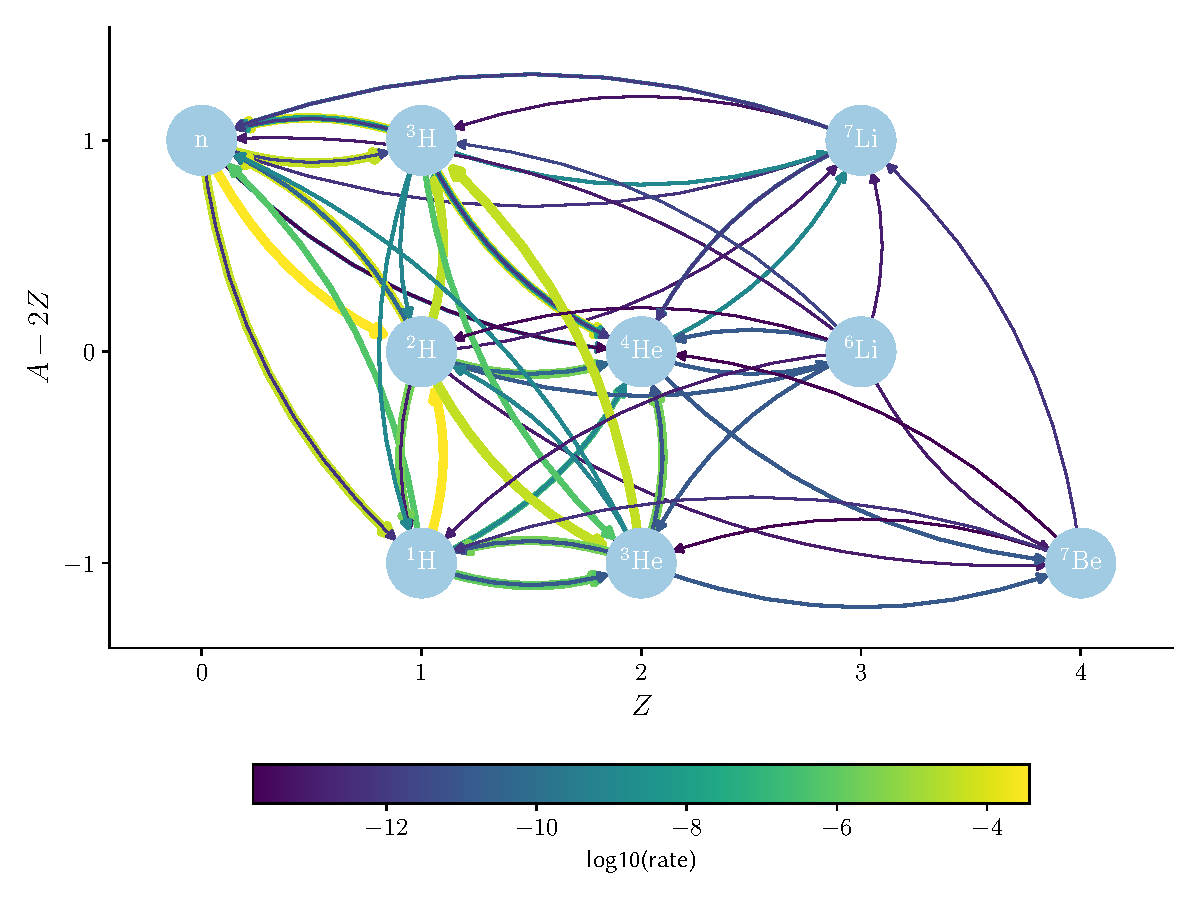
\includegraphics[height=10cm,trim={2cm 4.5cm 1cm 0},clip]{figures/smallnet5minutes.pdf}

    \vspace{1cm}

    \fontsize{16pt}{20pt}\selectfont
    \spread{Hans Br{\"u}ner Dein}\par
    \spread{201706079}\par

    \bigskip

    \fontsize{14pt}{18pt}\selectfont
    \spread{Master's Thesis in Physics}\par
    \spread{February 2024}\par
    %\bigskip
    \vfill

    Supervisors: Thomas Tram \& Steen Hannested\par
    % \href{http://pure.au.dk/portal/da/persons/id(XXX).html}{NAVN} \par

    \vfill

    \fontsize{12pt}{14.5pt}\selectfont
    \href{https://www.phys.au.dk/}{Department of Physics and Astronomy}\par
    \href{https://www.au.dk/}{Aarhus University}

  \end{adjustwidth*}

  % Colophon
  \newpage
  \begin{adjustwidth*}{\frontpagecorrection}{-\frontpagecorrection}
    \thispagestyle{empty}
    \strut\vfill
    {
      \setlength{\parindent}{0pt}
      \addtolength{\parskip}{.6em}

      \begin{center}
        \bfseries\sffamily Colophon
      \end{center}

      \small

      \textsl{\projecttitle}

      {--- \textsl{\projecttitledanish}}

      \smallskip

      Master's thesis by Hans Br{\"u}ner Dein. Written under supervision by Asc.Prof. Thomas Tram \& Prof. Steen Hannested
      Department of Physics and Astronomy, Aarhus University.

      Typeset by the author with \LaTeX{} and the \textsf{memoir} document class,
      using Linux Libertine and Linux Biolinum {\fontandleading}.

      Printed at Aarhus University
    }
  \end{adjustwidth*}
\end{titlingpage}


% ~~~~~~~~~~~~~~~~~~~~~~~~~~~~~~~~~~~~~~~~~~~~~~~~~~~~~~~~~~~~~~~~~~~~~~~~~~~~~
% Abstracts
% ~~~~~~~~~~~~~~~~~~~~~~~~~~~~~~~~~~~~~~~~~~~~~~~~~~~~~~~~~~~~~~~~~~~~~~~~~~~~~
\thispagestyle{chapter}

% ~~~~~~~~~~~~~~~~~
% Abstract: English
% ~~~~~~~~~~~~~~~~~
\begin{multiabstract}{Abstract (English)} 
\noindent The goal of this thesis is to present the development of a new BBN code APODORA (Adaptable Python interface Offering Determination Of Relic Abundances). APODORA is designed to be more flexible than existing codes, with an emphasis on the use of modern standardized computing methods. Derivations of the equations describing the time evolution of various components in the early universe are presented. These are implemented in a flexible IPython environment with the reaction network being created using interfaces from pynucastro\cite{pynucastro2}. The numerical uncertainty associated with every relevant input parameter of the code is systematically examined to ensure a high level of numerical precision. An in-depth comparison between APODORA and \textsc{AlterBBN} is performed, demonstrating equal or superior precision and speed. Finally, the resulting final abundances from APODORA are compared with multiple existing BNN codes as well as observational data.

\end{multiabstract}


% ~~~~~~~~~~~~~~~~~
% Abstract: Danish
% ~~~~~~~~~~~~~~~~~
\plainbreak{2}

% Switch to Danish
\selectlanguage{danish}
\begin{multiabstract}{Resumé (Dansk)}
\noindent Målet med dette speciale er at præsentere udviklingen af en ny BBN-kode APODORA, (Adaptable Python interface Offering Determination Of Relic Abundances). APODORA er skabt med henblik på at være mere fleksible end eksisterende løsninger, men særlig fokus på anvendelsen af moderne og standardiserende løsningsmetoder. Udledning af ligningerne som beskriver tidsudviklingen af det tidlige univers bestanddele bliver præsenteret. Dette er implementeret i et fleksibelt IPython miljø, hvortil reaktionsnetværket bliver skabt ved hjælp af brugerflader fra pakken pynucastro\cite{pynucastro2}. Den numeriske usikkerhed forbundet med hver relevant inputparameter i koden undersøges systematisk, for at sikre et højt niveau af numerisk præcision. Der udføres en dybdegående sammenligning mellem APODORA og \textsc{AlterBBN}, som påviser at både hastighed og præcision er lige så god, hvis ikke bedre. Til sidst sammenlignes forudsigelserne fra APODORA med andre BNN-koder samt observationer.

\end{multiabstract}

% Reset document language to English
\selectlanguage{english}

% List of fixme-notes -- REMEMBER TO REMOVE!
%  --> When removed, things will end on the correct pages
\listoffixmes

% Preface (Danish: Forord)
% [comment-out if not required]
%% ============================================================================
%%
%%  Speciale / Master's thesis
%%
%%  Author: FORNAVN EFTERNAVN
%%
%%  Preface
%% ============================================================================

%\chapter{Preface}
%\label{chap:preface}

%\centering Acknowledgments

\begin{multiabstract}{Acknowledgements} 
\noindent First and foremost, I would like to thank my friends and family for supporting and believing in me throughout the entirety of my time at IFA. For this thesis, I would like to thank my supervisor Thomas Tram, and unofficial co-supervisor Steen Hannested, for helping me along the way and ensuring I reached the goal in the end. I would also like to thank Erik Steenberg, Camilla Sørensen, Emil Birk, and Marta Jensen for proofreading the first and second draft of this thesis. In addition, I want to thank all the people at 1520-823, and in particular Christiane Rahbek, for providing company during the long days and nights of writing this thesis. I would also like to thank the pynucastro team for being very helpful in quickly fixing bugs and adding necessary features, with special thanks to Michael Zingale. 

Finally, I would like to thank my grandfather for igniting the passion for science, which has led me to this moment.

\end{multiabstract}
%This thesis concludes my Master's degree in/at .....


% Table of contents
\clearpage
\tableofcontents*

% Introduction (as an actual chapter, but *without* a number)
% [comment-out if not required]
%% ============================================================================
%%
%%  Speciale / Master's thesis
%%
%%  Author: FORNAVN EFTERNAVN
%%
%%  Introduction
%% ============================================================================

\chapter{Introduction}
\label{chap:intro}

Everything we see around us is made of atoms, which at their core contain a nucleus. Atomic nuclei are the fundamental building blocks that make up the stars, planets, and the humans that live on them. Understanding the creation of atomic nuclei is to understand the origin of the world itself. 


\subsection*{A Brief History of Early Nucleosynthesis}
When the universe was only a microsecond old, quarks coalesced to form the first protons and neutrons\cite{NASAUniversehistory}. Initially, there was an equal amount of neutrons and protons, but as the universe cooled, the slightly lighter protons became favored. The neutrons and protons remained in thermal equilibrium until the universe cooled to around $10^{10}$K, a second after the Big Bang. Here, the interaction between neutrinos and baryons becomes too weak to maintain thermodynamic equilibrium, freezing the ratio of neutrons and protons at one to five. The protons and neutrons can fuse to create deuterium, but these nuclei are short-lived as their low binding energy makes them vulnerable to destruction by the abundant high-energy photons. As these photons cool, the average lifetime of deuterium increases,
giving the deuterium nuclei more time to combine into much more stable helium nuclei. The rate of helium creation increases until it becomes great enough to rapidly convert all available neutrons into helium at approximately 200 seconds. Due to the delay caused by deuterium, the temperature and density of the universe will be too low to create any more than trace amounts of heavier elements. And so, a few minutes after it began, primordial nucleosynthesis ends. Barring radioactive decay, the abundance of the various elements will remain unchanged until the first stars appear $10^8$ years later\cite{klessen2023firststars}. 
The first computer code describing this process was created by Robert Wagoner in the late sixties\cite{Wagoner67}. Since then, many others have followed, with each implementation having its advantages and disadvantages.
\clearpage
\section{Objective} 
The objective of this thesis is to create a new state-of-the-art BBN code from first principles. To differentiate this code from existing implementations, it must fulfill these five requirements:

\begin{itemize}
    \item \textbf{Accessibility}: The code needs to run on any machine without the use of any proprietary software or special environments. %To achieve this, my code will require nothing but Python 3.0 and publicly available packages.
    \item \textbf{Accuracy}: The results must be consistent with those of contemporary BBN codes. Additionally, the results must be internally consistent with well-constrained numerical errors. 
    \item \textbf{Alacrity}: The code must be as fast as other contemporary BBN codes.
    \item \textbf{Agnostic reaction rates}: The code should use nuclear reaction rates from a single publicly available database to avoid any bias in rate selection.
    \item \textbf{Adaptability}: The code should be flexible and allow the investigation of various physical processes without changing the basic structure.
\end{itemize}

\section{Outline}

This thesis has three main parts:

\noindent First we will go over the physics required to describe the Big Bang nucleosynthesis. This will entail deriving every necessary relation from fundamental equations of cosmology, statistical physics, and thermodynamics. 

\noindent Next, we will review the numerical implementation of BBN. We start by covering the history and numerical difficulties associated with BBN calculations. The implementation of APODORA will then be briefly discussed, including the steps taken to overcome the aforementioned numerical difficulties.


\noindent Finally, we will look at the results. First, we will look at how APODORA can be used to get an overview of the various nuclear processes during BBN. Then, we will discuss the numerical accuracy of the code and how different parameters influence the precision. Ultimately, we compare with the results of other codes and observations.





\subsubsection{Terminology}

In the later sections of the thesis, predicted values for various nuclear abundances will be shown. For historical reasons, these are usually given as a molar faction relative to the abundance of hydrogen. That is to say, the number of nucleons contained in the particular isotope relative to the amount of free protons. ${}^4$He is an exception and is instead expressed as a fraction of total nucleons and denoted by $Y_p$. Though not entirely accurate, both of these molar fractions are often referred to as mass fractions. 

As BBN represents a crossover of nuclear physics and astronomy, temperature is interchangeably measured in MeV and Kelvin. Here, it is helpful to remember MeV$=11.6\times10^9 $K or simply MeV$\approx 10^{10}$K.


%\textcolor{orange}{Her skal nok tilføjes mere, afhængigt af hvilke termer DIG, korrekturlæserne ikke kender :)}


% ~~~~~~~~~~~~~~~~~~~~~~~~~~~~~~~
% Mainmatter (the actual content)
% ~~~~~~~~~~~~~~~~~~~~~~~~~~~~~~~
\mainmatter

% Here the chapters are organised in individual files, but in the same folder.
% Another option is to make one folder per chapter. This can e.g. be useful if
% each chapter contains many figures.

% Chapter 1
%% ============================================================================
%%
%%  Master's thesis
%% 
%%  Author: FORNAVN EFTERNAVN
%%
%%  Chapter 1: Coffee
%% ============================================================================

\chapter{BBN physics and cosmology}
\label{chap:theory}

This will be about the physics of BBN.

% ~~~~~~~~~~~~~~~~~~~~~~~~~~~~~~~~~~~~~~~~~~~~~~~~~~~~~~~~~~~~~~~~~~~~~~~~~~~~~
% SECTION
% ~~~~~~~~~~~~~~~~~~~~~~~~~~~~~~~~~~~~~~~~~~~~~~~~~~~~~~~~~~~~~~~~~~~~~~~~~~~~~
\section{cosmology}
\label{sec:cosmology}

citation test\textcite{kww}

\subsection{Electron/positron density and pressure}

\lipsum


% ~~~~~~~~~~
% SUBSECTION
% ~~~~~~~~~~
\subsection{Nuclear reactions}
\label{sec:nucleartheory}

Warning test\fxwarning{This is a warning!}

\lipsum


% Chapter 2
%% ============================================================================
%%
%%  Master's thesis
%%
%%  Author: FORNAVN EFTERNAVN
%%
%%  Chapter 2: Another topic....
%% ============================================================================

\chapter{BBN code}
\label{chap:BBNcode}

\section{History of BBN codes}
\label{sec:BBN_history}

The concept of Big Bang nucleosynthesis is almost as old as the Big bang theory itself, with the with it first being proposed in the paper by \cite{Gamov48}. However interest waned, as stellar nucleosynthesis proved itself much more useful in explaining present element abundances. 

With the discovery of the CMB in 1965, new attention was brought to the early universe. Only a year later Peebles showed how simple BBN physics could be used to explain the high helium abundance, unaccounted for by stellar nucreosynthesis \cite{Peebles66}. Soon after Wagoner created and refined the first proper bbn code, described in a series of classic papers \cite{Wagoner67} \cite{Wagoner69} \cite{Wagoner72}.


By the late 80's the wagoner code was severly outdated. With multiple ineffeciencies due to among other things, the fact that it was originally designed to run on punch cards. This inspired Lawrence Kawano to create the now ubiquitous NUC123, colloquially know as the Kawano code. Which set the gold Standard for all future BBN codes. 



\subsection{Wagoner}
\label{sec:Wagoner}

\subsection{Kawano}
\label{sec:Kawano}

\subsection{Modern codes}
\label{sec:Modern_codes}
PArthENoPE, AlterBBN, PRIMAT


\subsection{AlterBBN}
\label{sec:AlterBBN}

AlterBBN is written in c and based on Kawano's NUC123. It maintains the same basic structure and integration method, though it uses natural units for everything but the reaction network. However they defines energy in GeV rather than MeV. What seperates AlterBBN for other codes is that as the name implies, it allows the use of alternate cosmological models and parametes. Therefore this code is especially well suited for testing the effects these alterrations have on final abundances.


% Chapter 1
\chapter{Comparison with AlterBBN}
\label{chap:Alter}





\section{Types of Coffee}
\label{sec:intro_alter}

% ~~~~~~~~~~~~
% Bibliography
% ~~~~~~~~~~~~
\clearpage

% Change the sorting of references to NAME-YEAR-TITLE (see preamble for details)
\begin{refcontext}[sorting=nyt]
  % Standard bibliography
  \raggedyright[4em] \printbibliography

  % With custom title (activate in preamble)
  % \raggedyright[4em] \printbibliography[heading=memoirbib]
\end{refcontext}


% ~~~~~~~~~~
% Appendices
% ~~~~~~~~~~
%\appendix
%\chapter{Additional plots}
\label{chap:more_plots}

\begin{figure}[ht]
    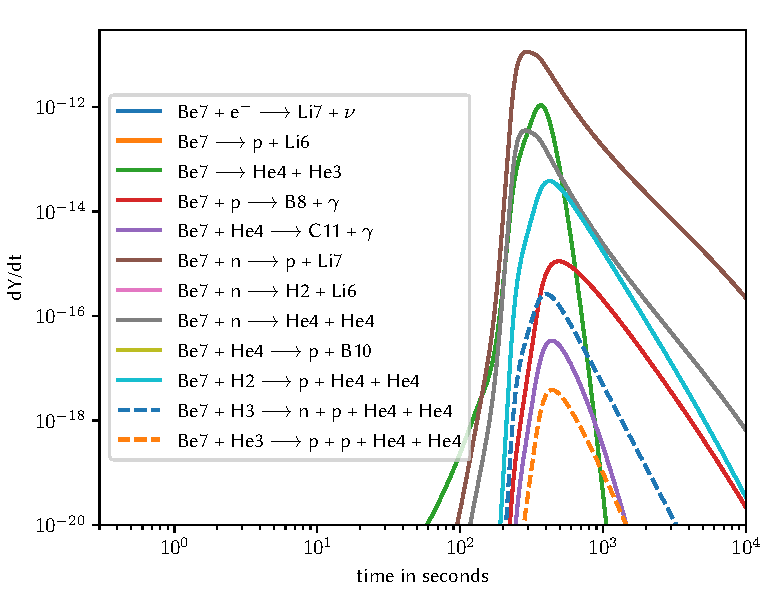
\includegraphics[width=5.1in]{figures/app/Be7destruct.pdf}
    \caption{Strength of different ${}^7$ Be destruction rates}
    \label{fig:Be7destruct}
\end{figure}

\begin{figure}[ht]
    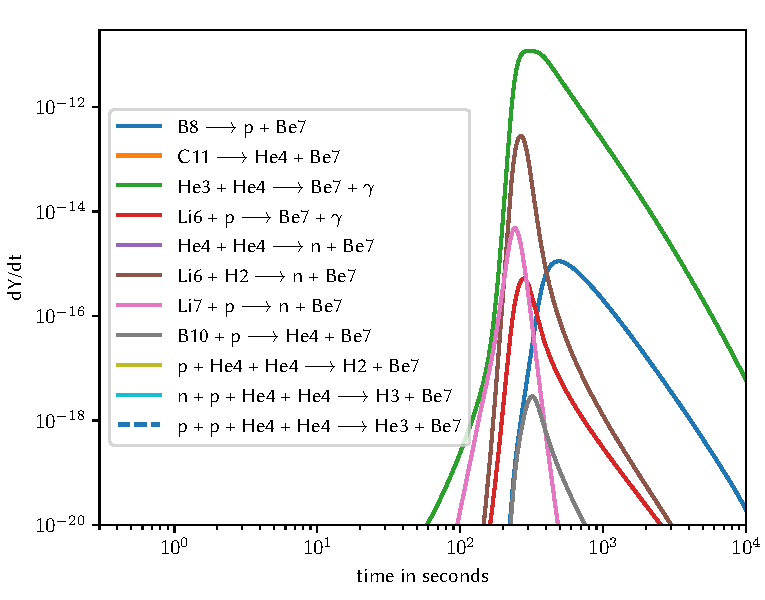
\includegraphics[width=5.1in]{figures/app/Be7create.pdf}
    \caption{Strength of different ${}^7$ Be creation rates}
    \label{fig:Be7create}
\end{figure}

\begin{figure}[ht]
    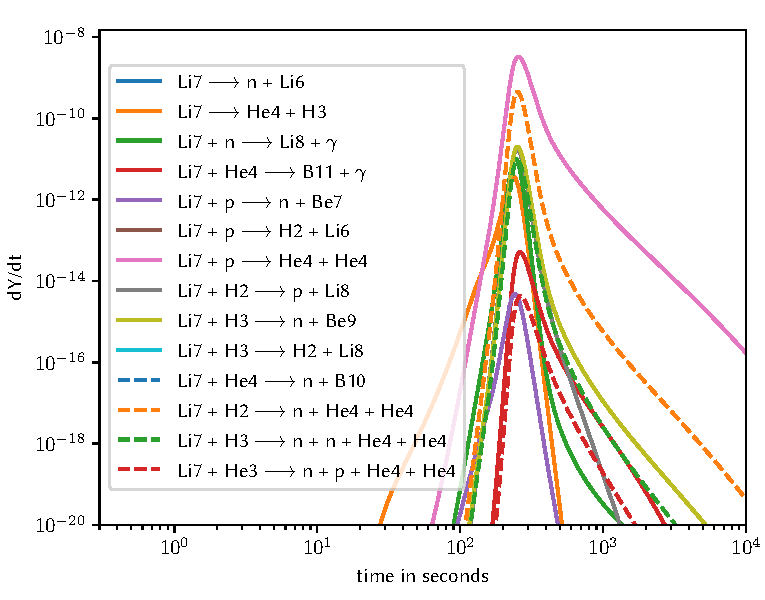
\includegraphics[width=5.1in]{figures/app/Li7destruct.pdf}
    \caption{Strength of different ${}^7$ Li destruction rates}
    \label{fig:Li7destruct}
\end{figure}

\begin{figure}[ht]
    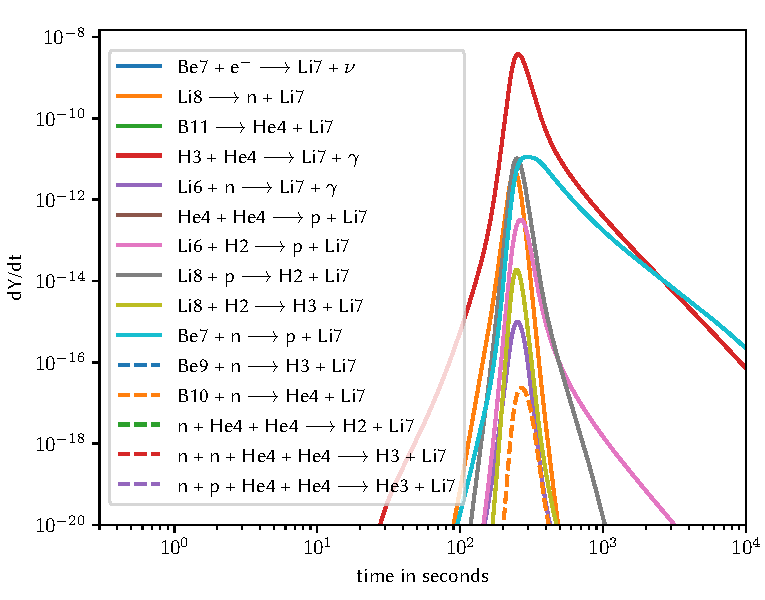
\includegraphics[width=5.1in]{figures/app/Li7create.pdf}
    \caption{Strength of different ${}^7$ Li creation rates}
    \label{fig:Li7create}
\end{figure}

\end{document}